\documentclass[11pt,a4paper]{scrartcl}

\usepackage[utf8]{inputenc}
\usepackage[T1]{fontenc}
\usepackage[lithuanian]{babel}
\usepackage{amsmath, amssymb, amsthm}
\usepackage{tikz}
\usetikzlibrary{angles,quotes,calc,decorations.markings,intersections}
\usepackage{geometry}
\geometry{margin=2cm}

\title{\Large Geometrijos Lapelis: Kampų Medžioklės Pradžiamokslis}
\author{Metodika: „Listokų“ sistema ir įrodymo menas}
\date{}

\begin{document}

\maketitle

\section*{Naujos žaidimo taisyklės}

Nuo šiol pamirštame mokyklinį įprotį „matlankiu pamatuoti brėžinį“ ar rašyti atsakymus be jokio paaiškinimo. Šis lapelis skirtas \textbf{kampų medžioklei} (\textit{Angle Chasing}) – metodui, kai naudodamiesi vos keliomis bazinėmis taisyklėmis, nežinomus kampus pažymime raidėmis (\(\alpha, \beta, \gamma\)) ir perkeliame jas po visą brėžinį.

\textbf{Svarbiausia taisyklė:} Kiekvienas jūsų teiginys privalo turėti geometrinį pagrindimą. Visus uždavinius iš pradžių apginkite mokytojui žodžiu, o tik tuomet tvarkingai užrašykite lape naudodami žodynėlį.

\vspace{0.5cm}
\noindent\fbox{%
    \parbox{\textwidth}{%
        \textbf{Privalomas įrodymų žodynėlis:}
        \begin{itemize}
            \item \textbf{Pradžia:} \textit{„Tarkime, kad...“}, \textit{„Pažymėkime...“}
            \item \textbf{Tikslo deklaravimas:} \textit{„Mūsų tikslas – parodyti, kad...“}, \textit{„Norint tai įrodyti, pakanka įsitikinti, jog...“}
            \item \textbf{Loginės jungtys:} \textit{„Pagal uždavinio sąlygą...“}, \textit{„Remdamiesi lygiašonio trikampio savybe...“}, \textit{„Kadangi tiesės lygiagrečios, susidarę vidaus priešiniai kampai yra lygūs...“}
            \item \textbf{Išvados:} \textit{„Iš to išplaukia, kad...“}, \textit{„Vadinasi,...“}, \textit{„Ką ir reikėjo įrodyti (k. r. į.).“}
        \end{itemize}
    }%
}
\vspace{0.5cm}

% ==========================================
% I DALIS
% ==========================================
\section*{I DALIS: Apšilimas ir Griežta Kalba (1–3 uždaviniai)}

\textbf{1 (Formalizavimo treniruotė).} Lygiašonio trikampio \(ABC\) (\(AB=BC\)) išorinis kampas prie viršūnės \(A\) lygus \(140^\circ\). Apskaičiuokite visus trikampio \(ABC\) vidaus kampus. \\
\textit{Reikalavimas:} Aprašykite sprendimą pilnais sakiniais, nurodydami, kodėl kiekvienas kampas yra būtent toks (naudokite gretutinių kampų ir lygiašonio trikampio savybes bei privalomąsias frazes).

\vspace{0.5cm}

\textbf{2 (Detektyvas: Rask klaidą).} \\
\textit{Sąlyga:} Trikampyje \(ABC\) kampas \(\angle A = 50^\circ\), o kampas \(\angle B = 70^\circ\). Iš viršūnės \(B\) išvesta aukštinė \(BD\). Apskaičiuokite kampą \(\angle ABD\).\\
\textit{Jono sprendimas:} „Kadangi trikampio kampų suma 180, tai \(\angle C = 180 - 50 - 70 = 60\). Aukštinė dalija kampą per pusę, todėl \(\angle ABD = 70 / 2 = 35^\circ\). Atsakymas 35.“\\
\textit{Jūsų užduotis:} Jonas gavo 0 taškų. Raskite grubią loginę klaidą Jono samprotavime (ko automatiškai negalima daryti su aukštine, nebent trikampis yra ypatingas?) ir parašykite \textbf{teisingą} sprendimą.

\vspace{0.5cm}

\textbf{3 (Įrodymo griaučiai: Euklido laužtė).} Tarp dviejų lygiagrečių tiesių \(a\) ir \(b\) nubrėžta laužtė. Pažymėję prie tiesių esančius smailiuosius kampus \(\alpha\) ir \(\beta\), \textbf{užpildykite įrodymo spragas}, kad įrodytumėte, jog kampas laužtės „smaigalyje“ lygus \(\alpha + \beta\).
\begin{center}
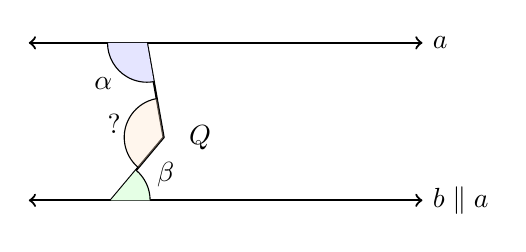
\begin{tikzpicture}[scale=1]
    \coordinate (A1) at (0,2); \coordinate (A2) at (5,2);
    \coordinate (B1) at (0,0); \coordinate (B2) at (5,0);
    \draw[thick, <->] (A1) -- (A2) node[right] {\(a\)};
    \draw[thick, <->] (B1) -- (B2) node[right] {\(b \parallel a\)};
    \coordinate (P) at (1.5,2);
    \coordinate (Q) at (1.712,0.8);
    \coordinate (R) at (1.041,0);
    \draw[thick] (P) -- (Q) -- (R);
    \pic[draw, fill=blue!10, "\(\alpha\)", angle radius=5mm, angle eccentricity=1.1,
        pic text options={text=black,text opacity=1,xshift=-2mm, yshift=-1mm}] {angle=A1--P--Q};
    \pic[draw, fill=green!10, "\(\beta\)", angle radius=5mm, angle eccentricity=1.1,
        pic text options={text=black,text opacity=1,xshift=2mm, yshift=1mm}] {angle=B2--R--Q};
    \pic[draw, fill=orange!20, fill opacity=0.35, "?", angle radius=5mm, angle eccentricity=1.3,
        pic text options={text=black,text opacity=1}] {angle=P--Q--R};
    \node[right=2mm] at (Q) {\(Q\)};
\end{tikzpicture}
\end{center}
\textit{Sprendimo griaučiai:}
„\textbf{Mūsų tikslas – parodyti, kad} kampas ties viršūne \(Q\) lygus \(\alpha + \beta\). \textbf{Norint tai įrodyti, pakanka} per tašką \(Q\) nubrėžti pagalbinę tiesę \(c\), lygiagrečią abiem duotoms tiesėms (\(c \parallel a\) ir \(c \parallel b\)).
Ši tiesė kampą padalija į dvi dalis. \textbf{Remdamiesi} lygiagrečių tiesių savybe, kad perkirtus jas kirstine, susidarantys vidaus priešiniai kampai yra ........................., matome, jog viršutinė kampo \(Q\) dalis lygi ..............., o apatinė dalis lygi ................
\textbf{Iš to išplaukia, kad} visas kampas \(Q\) yra lygus šių dviejų dalių sumai, t. y. ........................... \textbf{K. r. į.}“

\newpage
% ==========================================
% II DALIS
% ==========================================
\section*{II DALIS: Ginklų kalimas (4–6 uždaviniai)}
\textit{Šioje dalyje jūs patys įrodysite pagrindines teoremas. Vėlesniuose uždaviniuose jomis galėsite naudotis kaip „legaliais“ ginklais.}

\textbf{4 (Trikampio kampų suma).} Nusibraižykite bet kokį trikampį \(ABC\) ir jo vidinius kampus pažymėkite \(\alpha, \beta, \gamma\). Pasinaudodami 3-iojo uždavinio idėja (per vieną iš viršūnių nubrėžę tiesę, lygiagrečią priešingai kraštinei), \textbf{įrodykite}, kad:
\begin{equation*}
\alpha + \beta + \gamma = 180^\circ
\end{equation*}

\vspace{0.5cm}

\textbf{5 (Priekampio savybė).} Trikampio \(ABC\) kraštinė \(BC\) pratęsta už taško \(C\) (gaunamas išorinis kampas). \textbf{Mūsų tikslas – parodyti, kad} trikampio išorinis kampas (priekampis) visada yra lygus dviejų su juo negretimų vidaus kampų sumai. \textbf{Įrodykite} tai remdamiesi 4 uždavinio rezultatu ir gretutinių kampų savybe.

\vspace{0.5cm}

\textbf{6 („Bumerango“ lema).} Duotas neiškilusis keturkampis \(ABCD\). \textbf{Įrodykite}, kad jo įgaubtasis kampas \(\angle ADC\) lygus kitų trijų smailiųjų kampų sumai: \(\alpha + \beta + \gamma\). \\
\textit{Patarimas:} Pratęskite atkarpą \(AD\) tol, kol ji kirs priešingą kraštinę \(BC\). Tada du kartus pritaikykite ką tik įrodytą Priekampio savybę iš 5 uždavinio.
\begin{center}
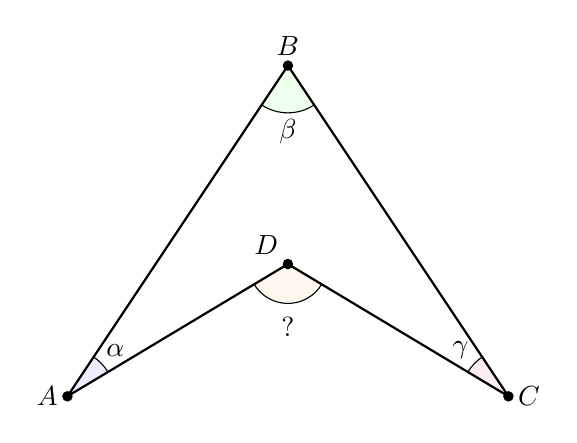
\begin{tikzpicture}[scale=1.4]
    \coordinate (A) at (-2,-1);
    \coordinate (B) at (0,2);
    \coordinate (C) at (2,-1);
    \coordinate (D) at (0,0.2);

    \pic[draw, fill=blue!20, fill opacity=0.35, "\(\alpha\)", angle radius=6mm, angle eccentricity=1.4, pic text options={text=black, text opacity=1}] {angle=D--A--B};
    \pic[draw, fill=green!20, fill opacity=0.35, "\(\beta\)", angle radius=6mm, angle eccentricity=1.4, pic text options={text=black, text opacity=1}] {angle=A--B--C};
    \pic[draw, fill=purple!20, fill opacity=0.35, "\(\gamma\)", angle radius=6mm, angle eccentricity=1.4, pic text options={text=black, text opacity=1}] {angle=B--C--D};
    \pic[draw, fill=orange!20, fill opacity=0.35, "?", angle radius=5mm, angle eccentricity=1.6, pic text options={text=black, text opacity=1}] {angle=A--D--C};

    \draw[thick] (A) -- (B) -- (C) -- (D) -- cycle;

    \foreach \p in {A,B,C,D} {\filldraw (\p) circle (1.2pt);}
    \node[left] at (A) {\(A\)};
    \node[above] at (B) {\(B\)};
    \node[right] at (C) {\(C\)};
    \node[above left] at (D) {\(D\)};
\end{tikzpicture}
\end{center}

% ==========================================
% III DALIS
% ==========================================
\section*{III DALIS: Pusiaukampinių paslaptys (7–9 uždaviniai)}
\textit{Pusiaukampinė dalija kampą per pusę. Tai reiškia, kad kampų medžioklėje visada atsiras trupmenos (pvz., \(\alpha/2\)). Nebijokite algebros!}

\textbf{7 (Aukštinė ir pusiaukampinė).} Trikampyje \(ABC\) nubrėžta aukštinė \(AH\) ir pusiaukampinė \(AD\). Žinoma, kad \(\angle B = 70^\circ\), o \(\angle C = 40^\circ\). \textbf{Apskaičiuokite} kampą tarp aukštinės ir pusiaukampinės (\(\angle HAD\)). Aprašykite sprendimą remdamiesi tiksliomis trikampių savybėmis.

\vspace{0.5cm}

\textbf{8 (Kampas tarp vidinių pusiaukampinių).} Trikampio \(ABC\) kampas \(\angle A = \alpha\). Iš viršūnių \(B\) ir \(C\) nubrėžtos pusiaukampinės susikerta taške \(I\). \textbf{Įrodykite}, kad kampas tarp jų visada išreiškiamas formule:
\begin{equation*}
\angle BIC = 90^\circ + \frac{\alpha}{2}
\end{equation*}
\textit{Patarimas:} Iš pradžių pažymėkite kampus \(\angle IBC = \beta\) ir \(\angle ICB = \gamma\). Trikampyje \(BIC\) išreikškite ieškomą kampą per \((\beta + \gamma)\). Tuomet pažiūrėkite į didįjį trikampį \(ABC\) ir išreikškite dydį \((\beta + \gamma)\) per \(\alpha\).

\begin{center}
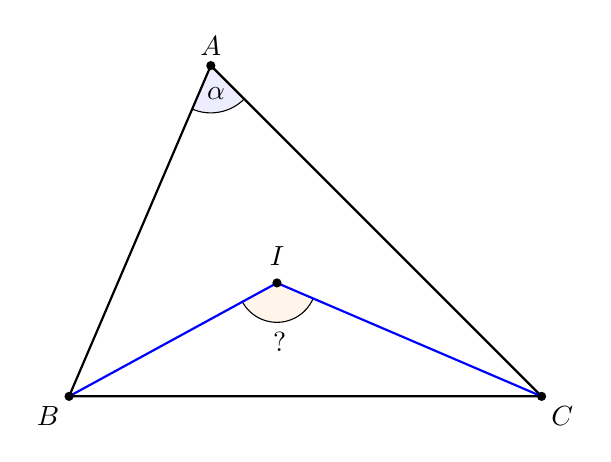
\begin{tikzpicture}[scale=1.2]
    \coordinate (B) at (0,0);
    \coordinate (C) at (5,0);
    \coordinate (A) at (1.5,3.5);
    \coordinate (I) at (2.2, 1.2);

    \pic[draw, fill=blue!20, fill opacity=0.35, "\(\alpha\)", angle radius=6mm, pic text options={text=black,text opacity=1}] {angle = B--A--C};
    \pic[draw, fill=orange!20, fill opacity=0.4, "?", angle radius=5mm, angle eccentricity=1.5, pic text options={text=black,text opacity=1}] {angle = B--I--C};

    \draw[thick] (A) -- (B) -- (C) -- cycle;
    \draw[thick, blue] (B) -- (I) -- (C);

    \foreach \p in {A,B,C,I} {\filldraw (\p) circle (1.2pt);}
    \node[above] at (A) {\(A\)};
    \node[below left] at (B) {\(B\)};
    \node[below right] at (C) {\(C\)};
    \node[above, yshift=1mm] at (I) {\(I\)};
\end{tikzpicture}
\end{center}

\vspace{0.5cm}

\textbf{9 (Kampas tarp išorinių pusiaukampinių).} Trikampio \(ABC\) \textbf{išorinių} kampų prie viršūnių \(B\) ir \(C\) pusiaukampinės susikerta taške \(J\). \textbf{Įrodykite}, kad:
\begin{equation*}
\angle BJC = 90^\circ - \frac{\angle A}{2}
\end{equation*}

\newpage
% ==========================================
% IV DALIS
% ==========================================
\section*{IV DALIS: Olimpiadinė klasika (10–12 uždaviniai)}
\textit{Čia reikės meistriškai apjungti lygiašonius trikampius, priekampius ir algebrines lygtis.}

\textbf{10 (Penkiakampė žvaigždė).} Nubraižykite bet kokią penkiakampę žvaigždę (sudarytą iš 5 atkarpų). Naudodamiesi priekampio savybe, visus penkis jos „smaigalių“ kampus perkelkite į vieno mažo trikampio vidų ir \textbf{įrodykite}, kad visų penkių kampų suma lygi \(180^\circ\).
\begin{center}
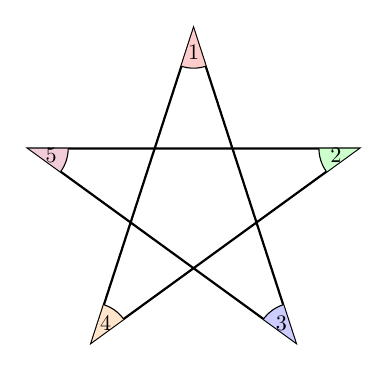
\begin{tikzpicture}[scale=1.1]
    \coordinate (P1) at (90:2);
    \coordinate (P2) at (18:2);
    \coordinate (P3) at (-54:2);
    \coordinate (P4) at (-126:2);
    \coordinate (P5) at (162:2);
    
    \draw[thick] (P1) -- (P3) -- (P5) -- (P2) -- (P4) -- cycle;
    
    \pic[draw, fill=red!20, "1", angle radius=5mm, pic text options={scale=0.8}] {angle=P4--P1--P3};
    \pic[draw, fill=green!20, "2", angle radius=5mm, pic text options={scale=0.8}] {angle=P5--P2--P4};
    \pic[draw, fill=blue!20, "3", angle radius=5mm, pic text options={scale=0.8}] {angle=P1--P3--P5};
    \pic[draw, fill=orange!20, "4", angle radius=5mm, pic text options={scale=0.8}] {angle=P2--P4--P1};
    \pic[draw, fill=purple!20, "5", angle radius=5mm, pic text options={scale=0.8}] {angle=P3--P5--P2};
\end{tikzpicture}
\end{center}

\vspace{0.5cm}

\textbf{11 (Kvadratas ir trikampis).} Kvadrato \(ABCD\) viduje ant kraštinės \(AB\) nubrėžtas lygiakraštis trikampis \(ABE\). \textbf{Apskaičiuokite} kampą \(\angle CDE\).\\
\textit{Patarimas:} Ieškokite paslėptų lygiašonių trikampių. Kraštinių ilgiai čia vaidina lemiamą vaidmenį (kvadrato kraštinė lygi lygiakraščio trikampio kraštinei!).

\vspace{0.5cm}

\textbf{12 (Auksinis trikampis).} Duotas lygiašonis trikampis \(ABC\), kurio kraštinės \(AB = AC\). Kraštinėje \(AC\) atidėtas taškas \(D\) taip, kad susidariusios atkarpos tenkina sąlygą \(AD = BD = BC\). 
\textbf{Įrodykite}, kad viršūnės kampas \(\angle A\) visada lygus lygiai \(36^\circ\).

\begin{center}
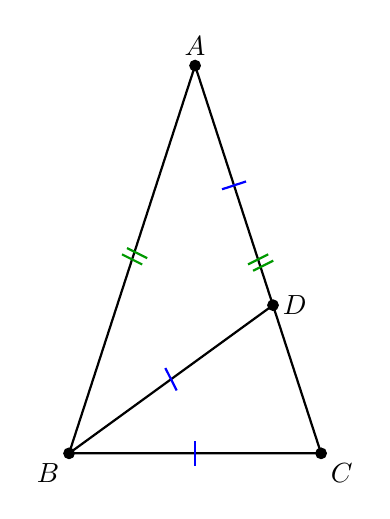
\begin{tikzpicture}[scale=1.6]
    \coordinate (B) at (0,0);
    \coordinate (C) at (2,0);
    \coordinate (A) at (1,3.077);
    \coordinate (D) at ($(A)!0.618!(C)$);

    \draw[thick] (A) -- (B) -- (C) -- cycle;
    \draw[thick] (B) -- (D);

    % Vienodi brūkšneliai pirmai grupei
    \draw[thick, blue] ($(A)!0.5!(D) + (-0.095, -0.031)$) -- ($(A)!0.5!(D) + (0.095, 0.031)$);
    \draw[thick, blue] ($(B)!0.5!(D) + (-0.045, 0.089)$) -- ($(B)!0.5!(D) + (0.045, -0.089)$);
    \draw[thick, blue] (1, -0.1) -- (1, 0.1);

    % Du brūkšneliai antrai grupei
    \coordinate (mAB) at ($(A)!0.5!(B)$);
    \draw[thick, green!60!black] ($(mAB) + (-0.08, 0.04)$) -- ($(mAB) + (0.08, -0.04)$);
    \draw[thick, green!60!black] ($(mAB) + (-0.04, 0.09)$) -- ($(mAB) + (0.12, 0.01)$);
    \coordinate (mAC) at ($(A)!0.5!(C)$);
    \draw[thick, green!60!black] ($(mAC) + (-0.08, -0.04)$) -- ($(mAC) + (0.08, 0.04)$);
    \draw[thick, green!60!black] ($(mAC) + (-0.04, -0.09)$) -- ($(mAC) + (0.12, -0.01)$);

    \foreach \p in {A,B,C,D} {\filldraw (\p) circle (1.2pt);}
    \node[above] at (A) {\(A\)};
    \node[below left] at (B) {\(B\)};
    \node[below right] at (C) {\(C\)};
    \node[right] at (D) {\(D\)};
\end{tikzpicture}
\end{center}
\textit{Įrodymo gairės (Nepraleiskite žingsnių!):} Pradėkite pažymėdami \(\angle A = \alpha\). Kadangi atkarpos rodo trikampių lygybes, ieškokite lygiašonių trikampių (pirmiausia \(\triangle ADB\), po to \(\triangle BDC\), galiausiai pats \(\triangle ABC\)). Prisiminkite priekampio savybę. Išreiškę visus trikampio \(ABC\) kampus per dydį \(\alpha\), sudarykite kampų sumos lygtį ir ją išspręskite.

\end{document}